\newpage
\appendix

\section{Qualitative Analysis}
\label{sec:qualitative}
In this section, we provide more qualitative analyses on most valuable data identified by \method. In particular, we show top-2$\sim$4 valuable data for each query here, given the possibility that the model utilizes information from multiple training examples for generating its output. We also include several failure cases where identified most valuable data do not share qualitative similarities with the queried LLM output.

\subsection{Llama3-8B-Instruct}

\subsubsection{Example 1}
\begin{figure}[htbp]
    \centering
    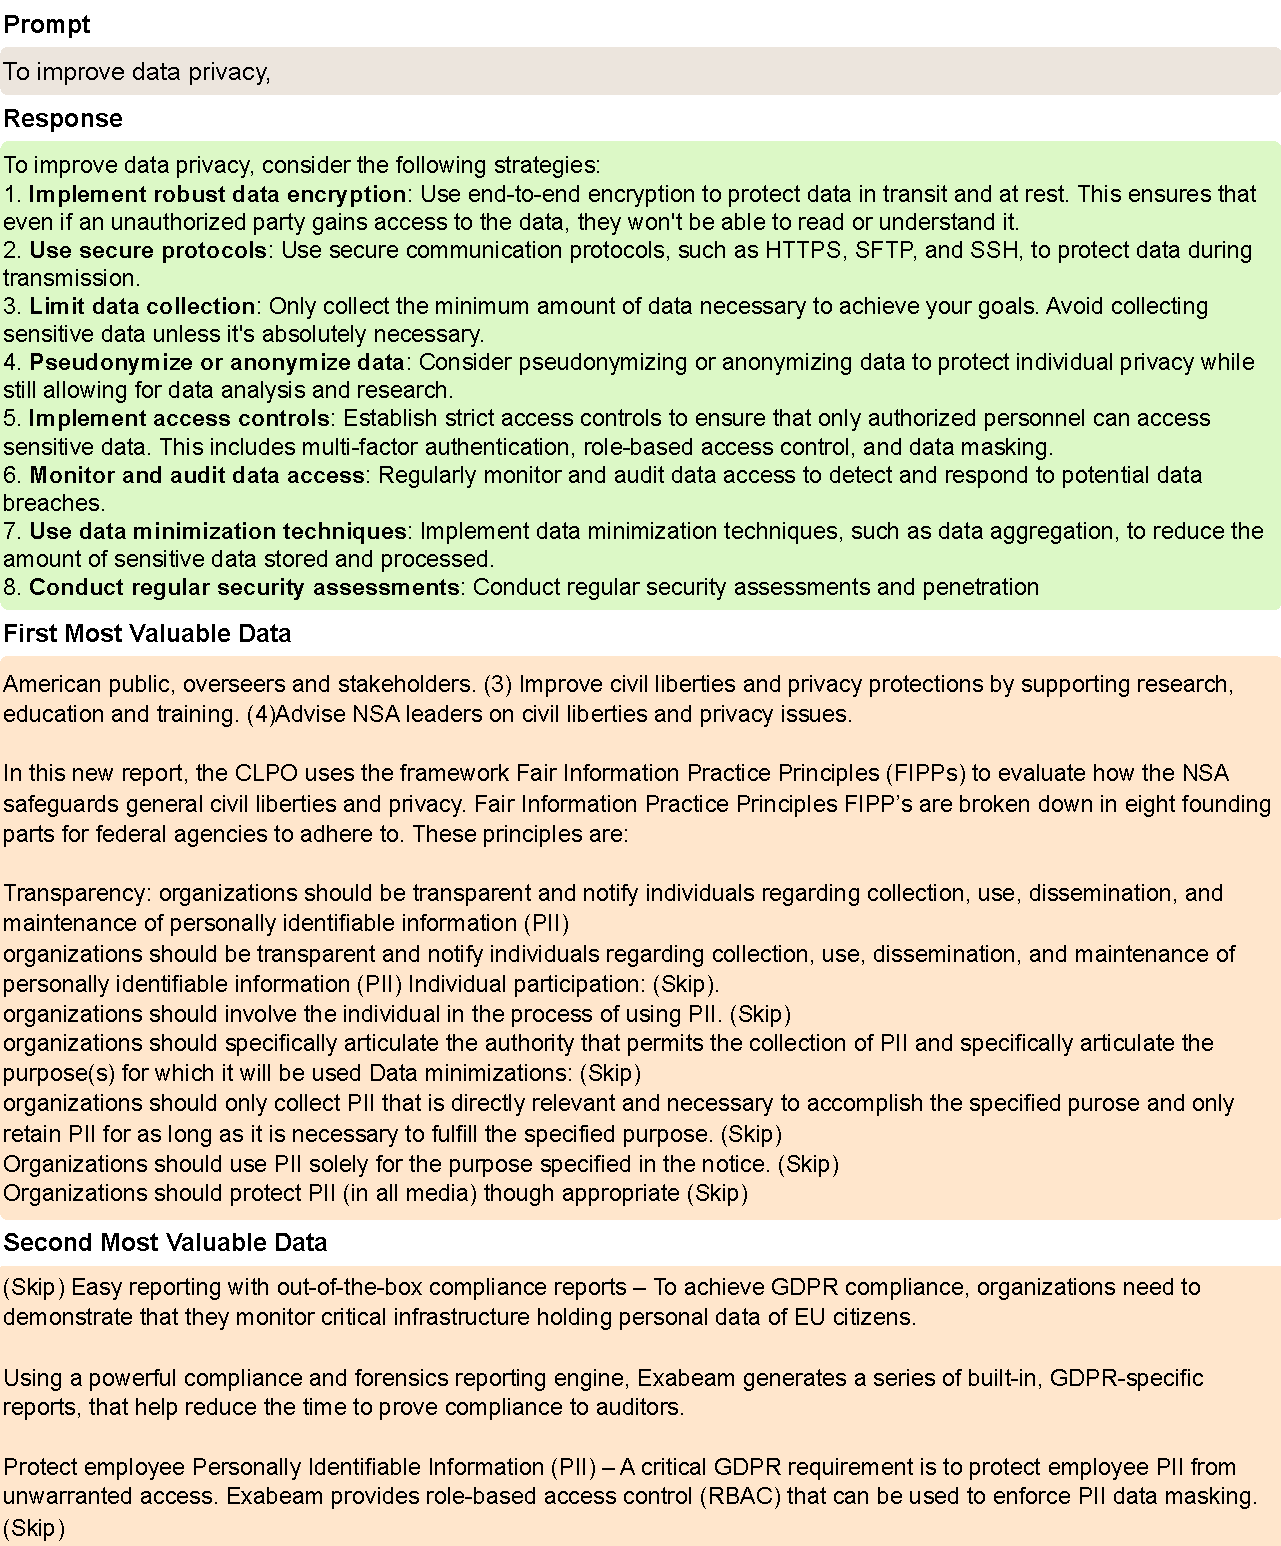
\includegraphics[width=0.99\textwidth]{figures/llama3_appendix1.pdf}
    \caption{Llama3-8B-Instruct data valuation result.}
\end{figure}

\clearpage
\subsubsection{Example 2}

\begin{figure}[htbp]
    \centering
    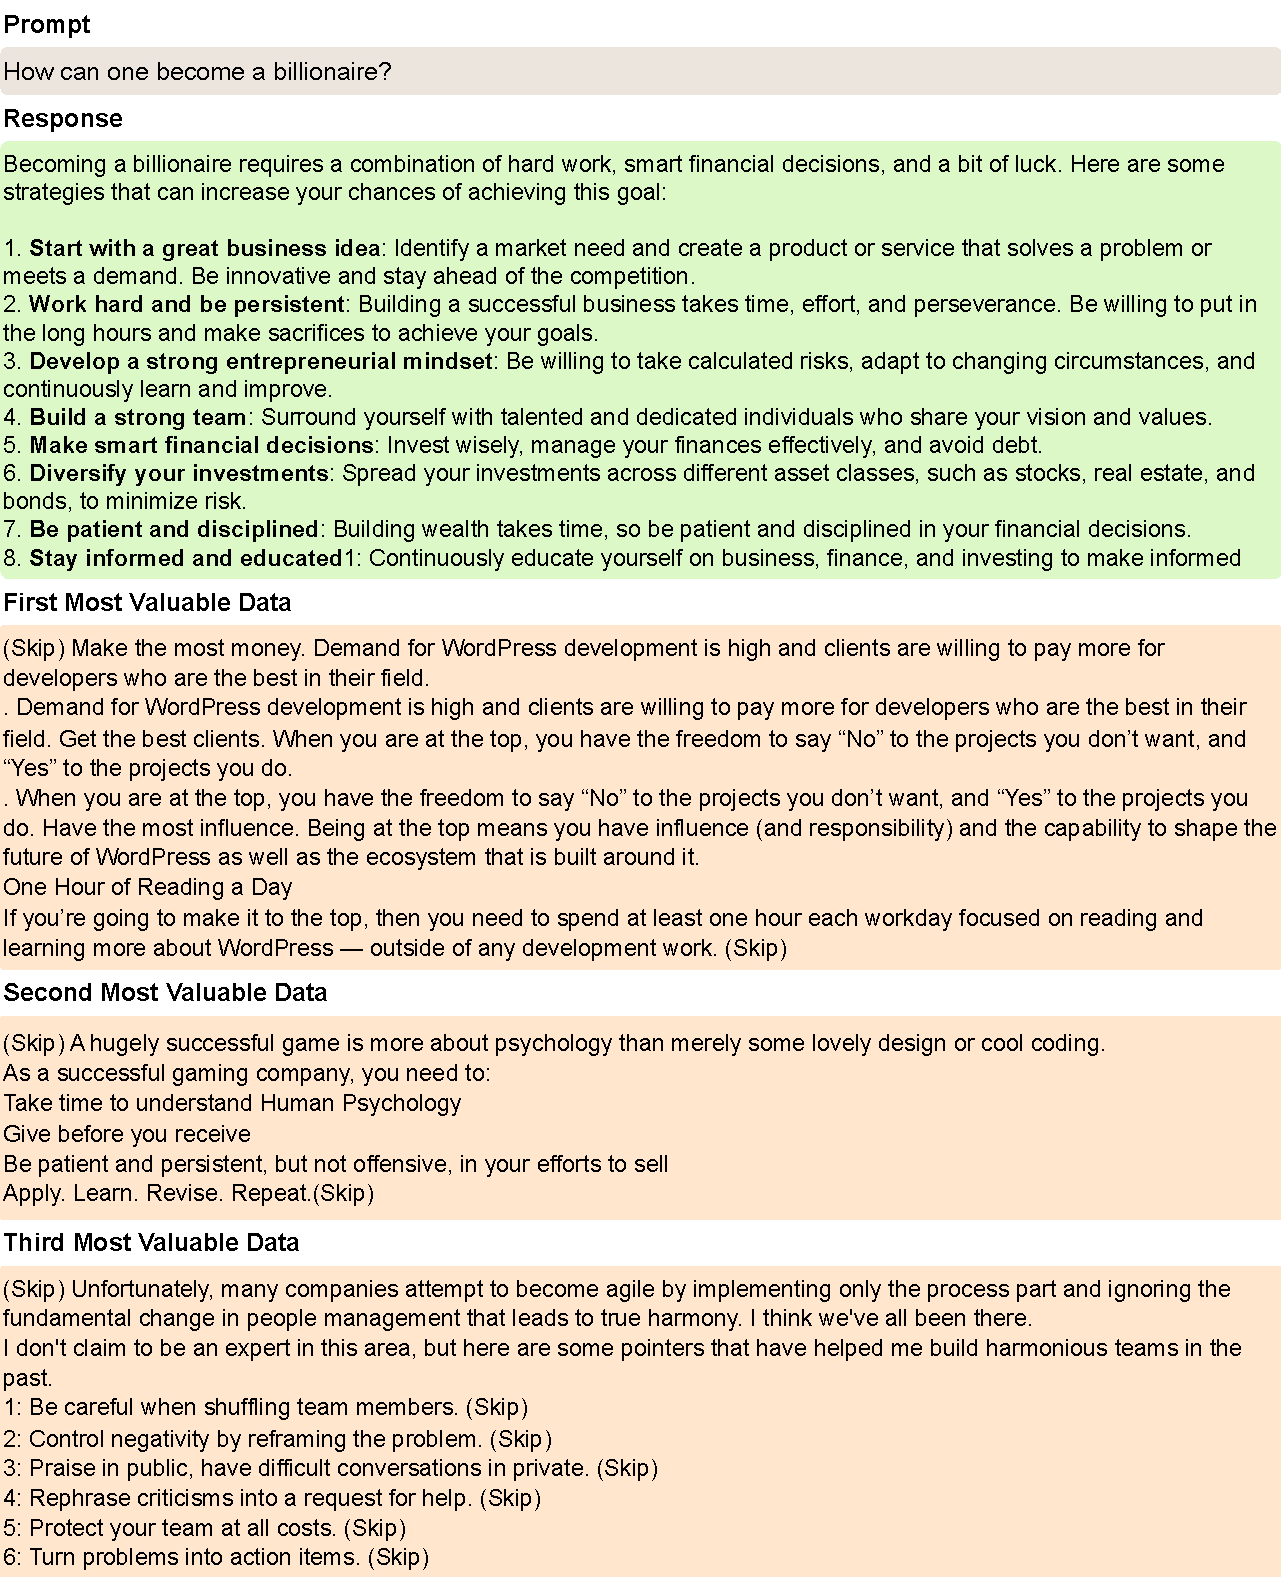
\includegraphics[width=0.99\textwidth]{figures/llama3_appendix2.pdf}
    \caption{Llama3-8B-Instruct data valuation result.}
\end{figure}

\clearpage
\subsubsection{Example 3}

\begin{figure}[htbp]
    \centering
    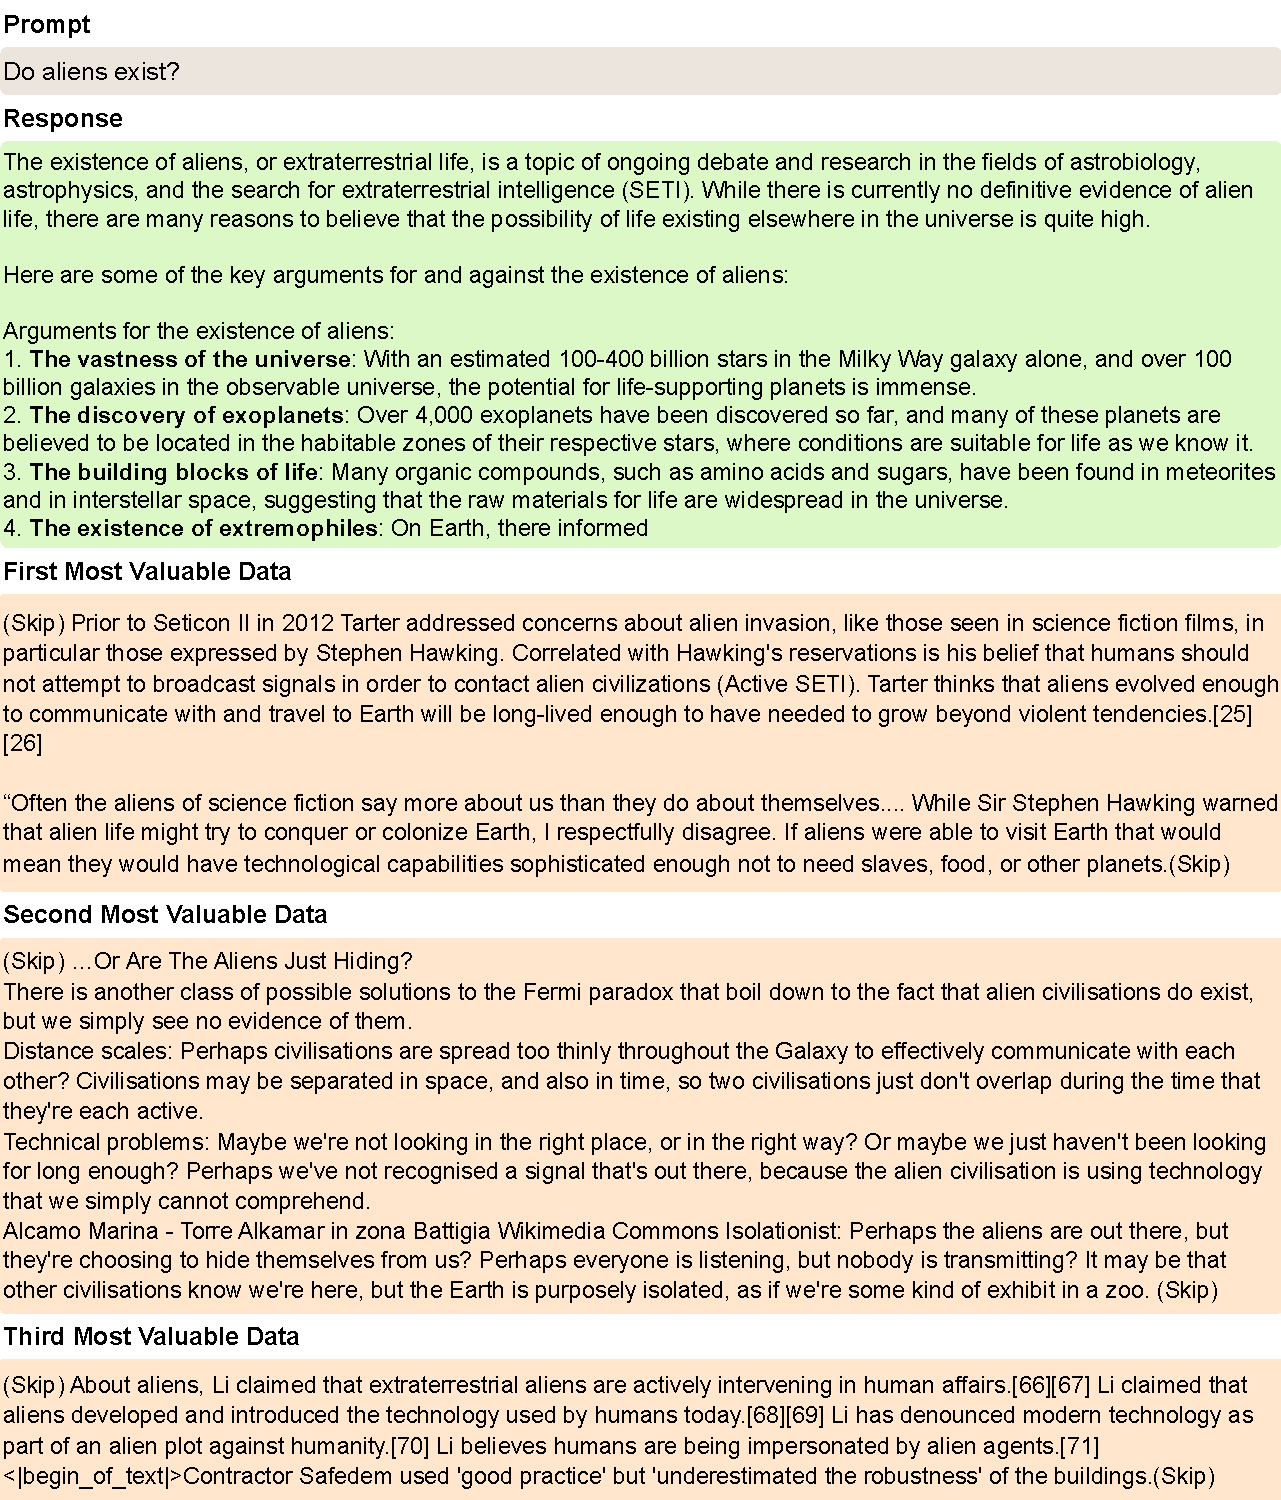
\includegraphics[width=0.99\textwidth]{figures/llama3_appendix3.pdf}
    \caption{Llama3-8B-Instruct data valuation result.}
\end{figure}

\clearpage
\subsubsection{Example 4}

\begin{figure}[htbp]
    \centering
    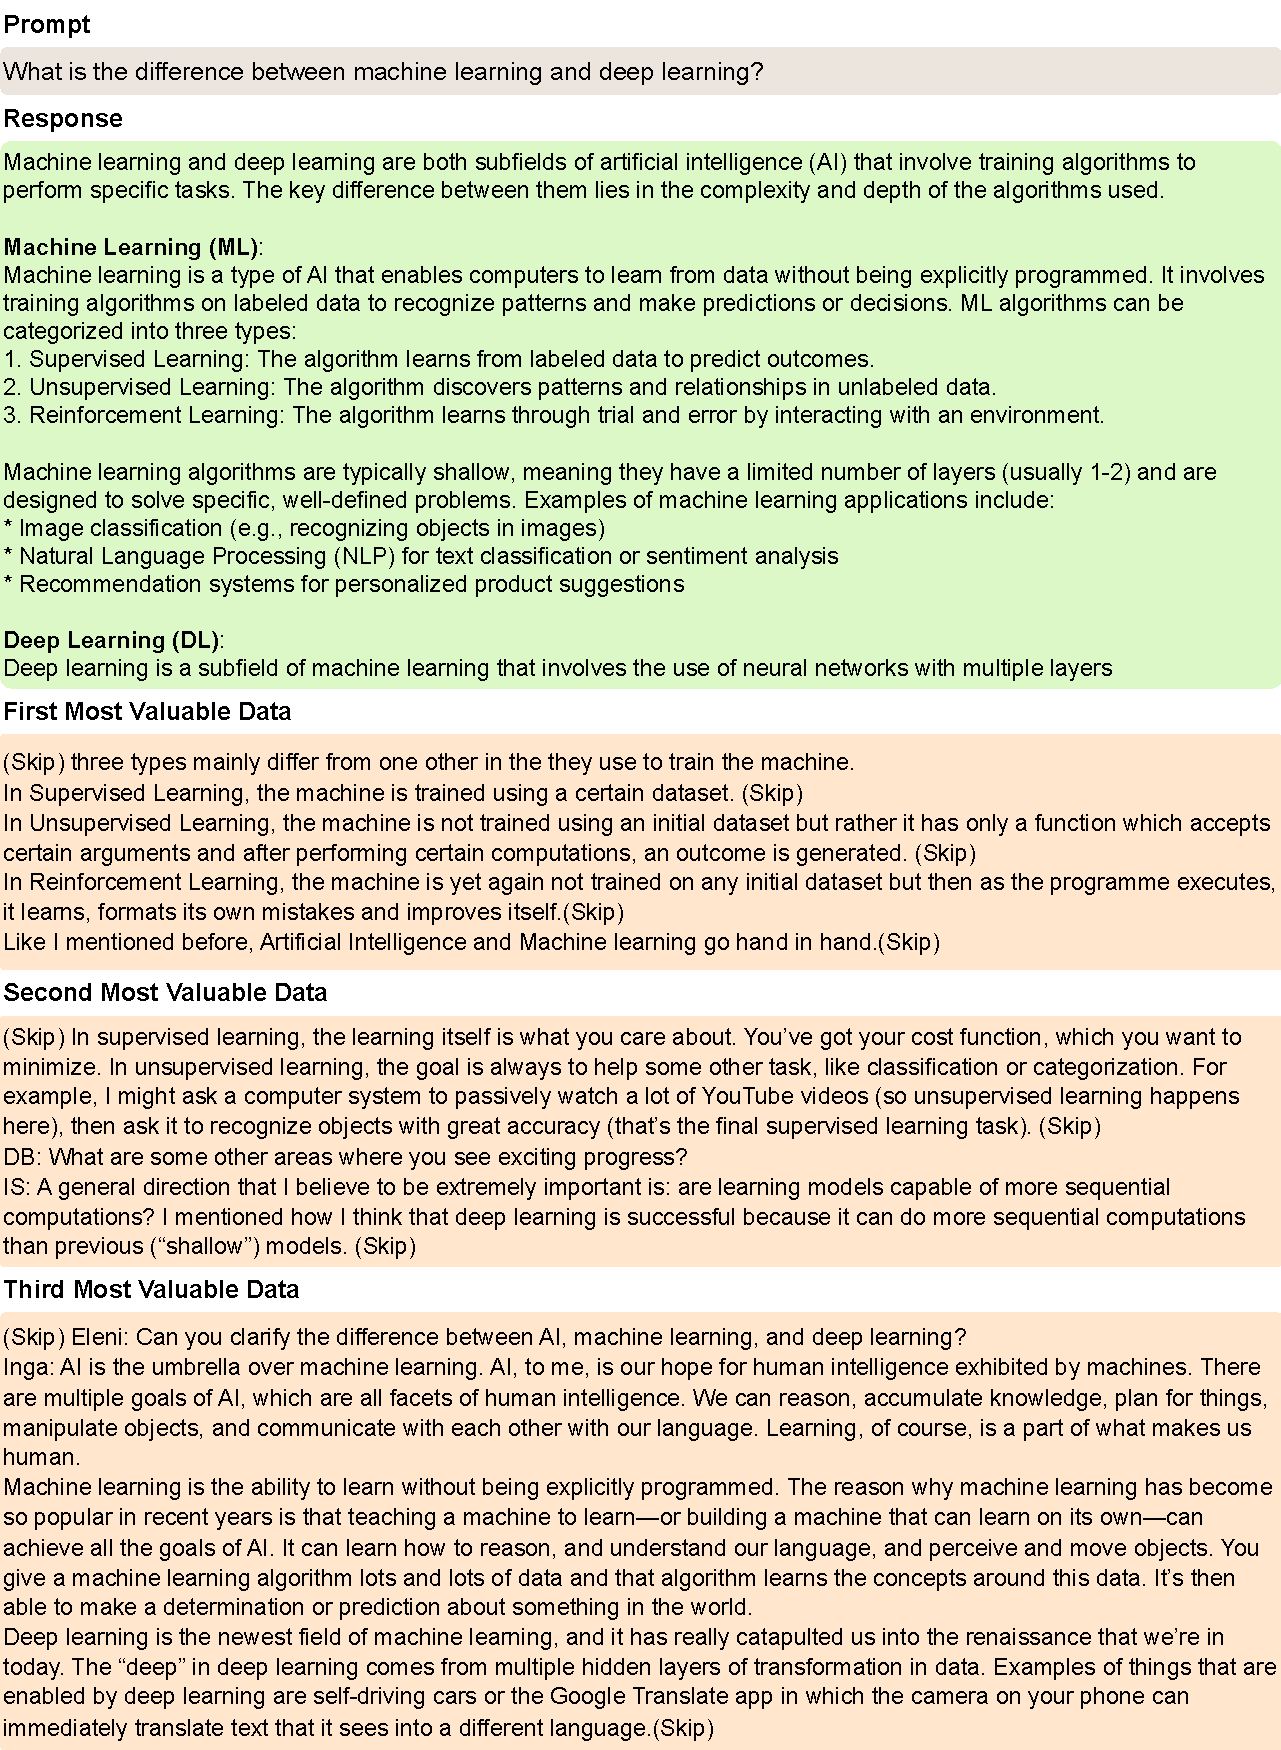
\includegraphics[width=0.99\textwidth]{figures/llama3_appendix4.pdf}
    \caption{Llama3-8B-Instruct data valuation result.}
\end{figure}

\clearpage
\subsubsection{Example 5}

\begin{figure}[htbp]
    \centering
    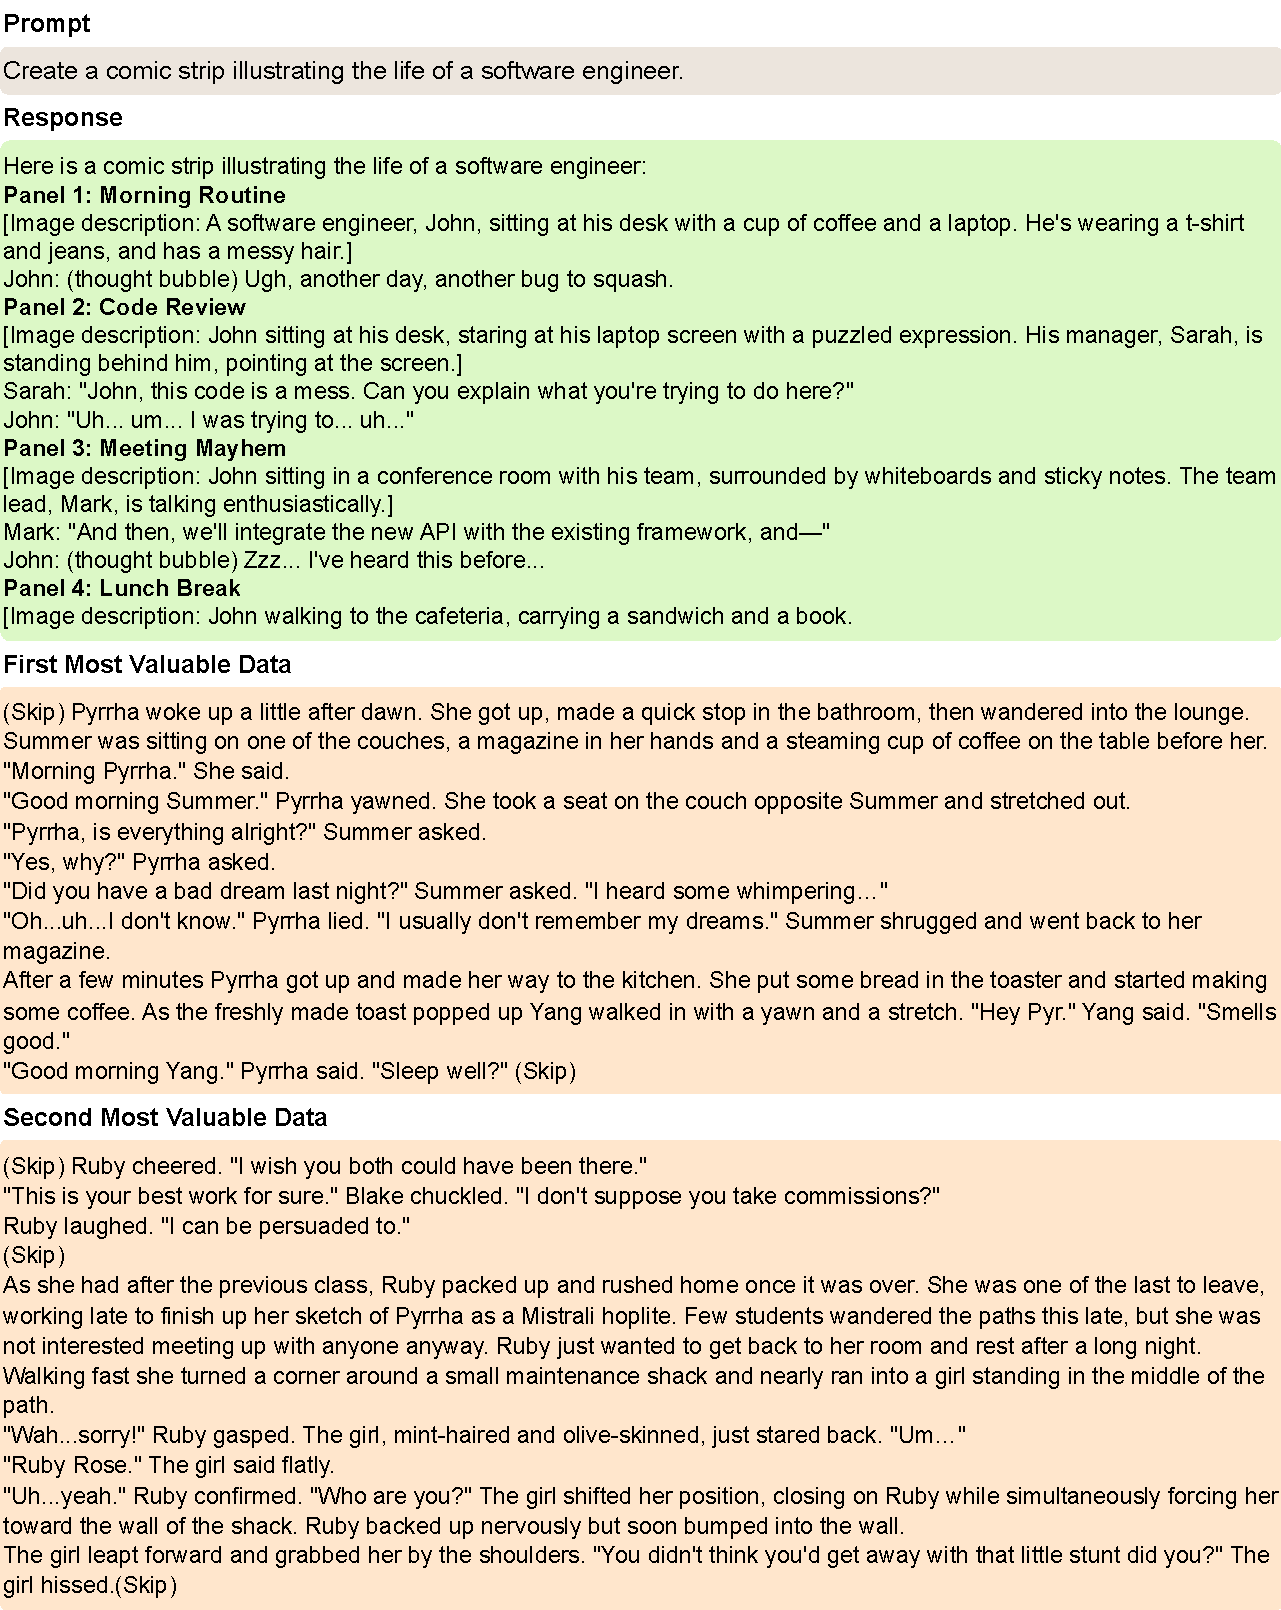
\includegraphics[width=0.99\textwidth]{figures/llama3_appendix5.pdf}
    \caption{Llama3-8B-Instruct data valuation result. \method\ identifies novel literature as most valuable data.}
\end{figure}

\clearpage
\subsubsection{Example 6 (Failure)}

\begin{figure}[htbp]
    \centering
    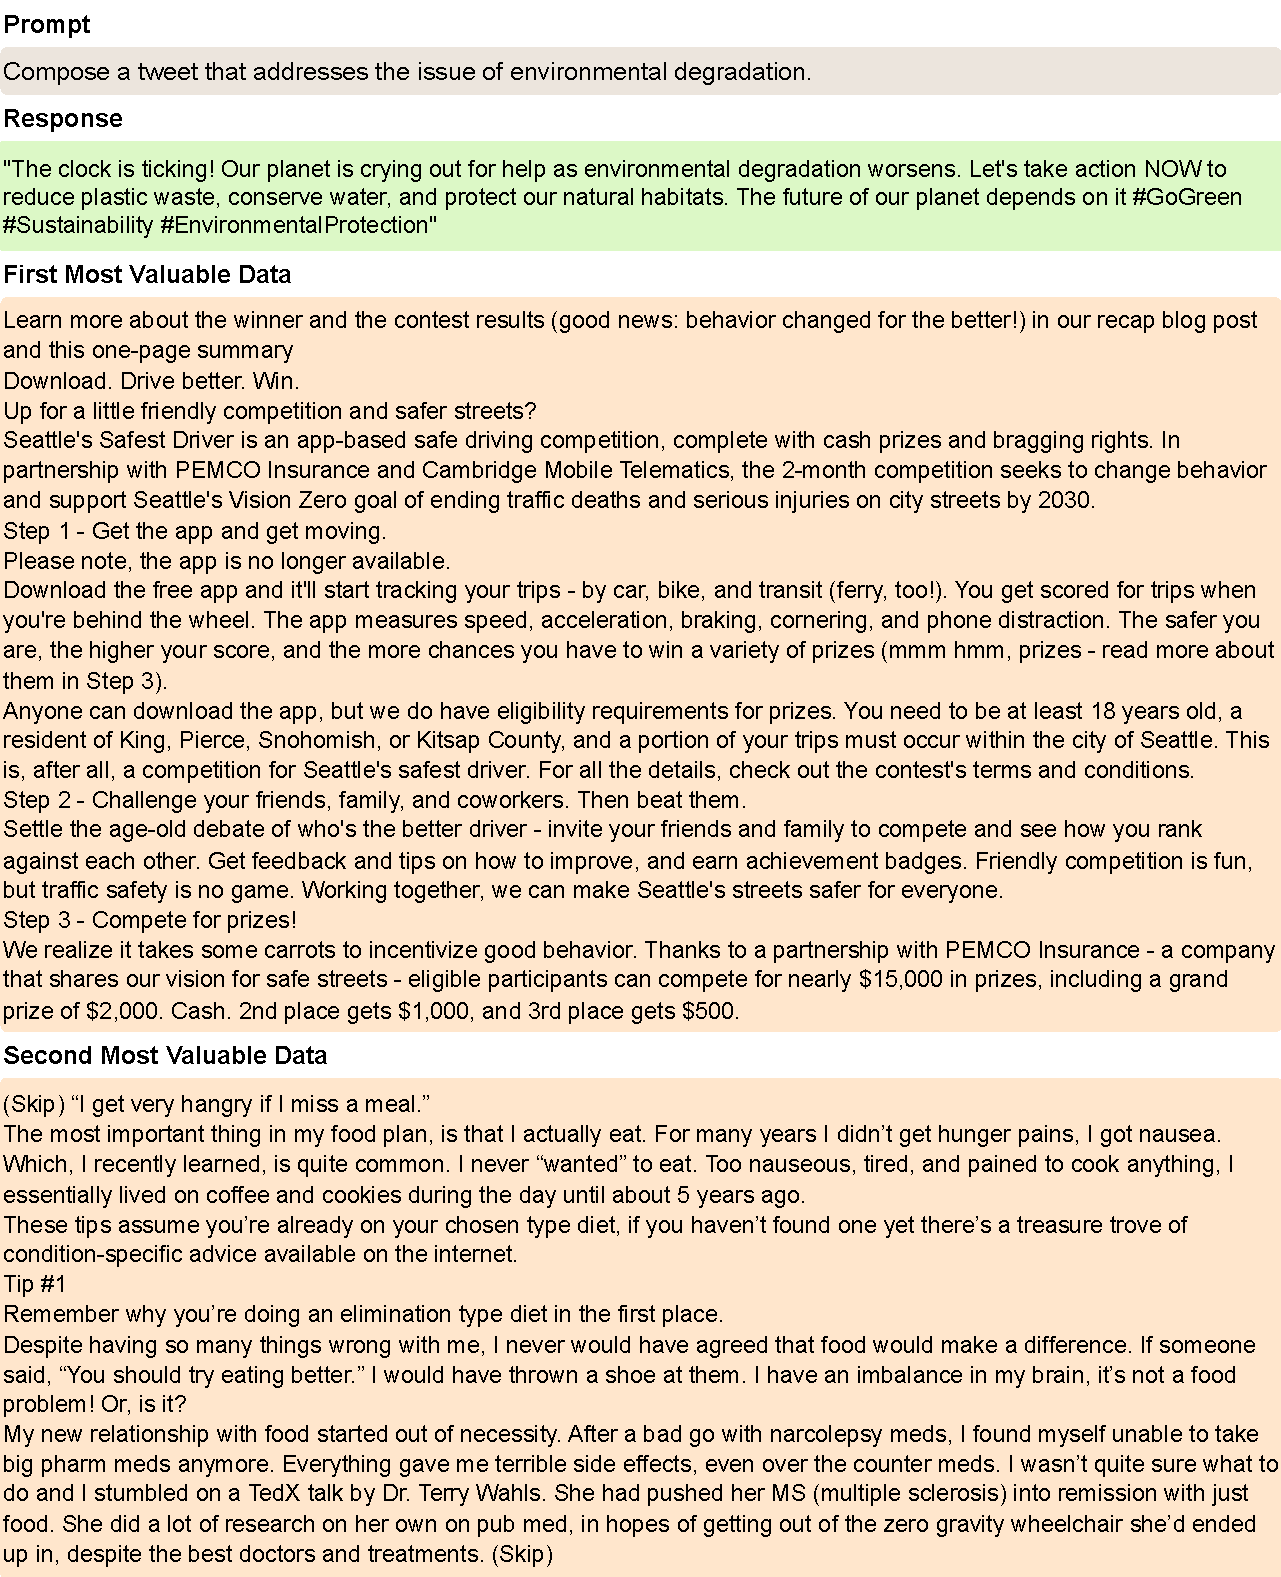
\includegraphics[width=0.99\textwidth]{figures/llama3_appendix6.pdf}
    \caption{Llama3-8B-Instruct data valuation result.}
\end{figure}

\clearpage

\subsection{GPT2-XL}

\subsubsection{Example 1}

\begin{figure}[htbp]
    \centering
    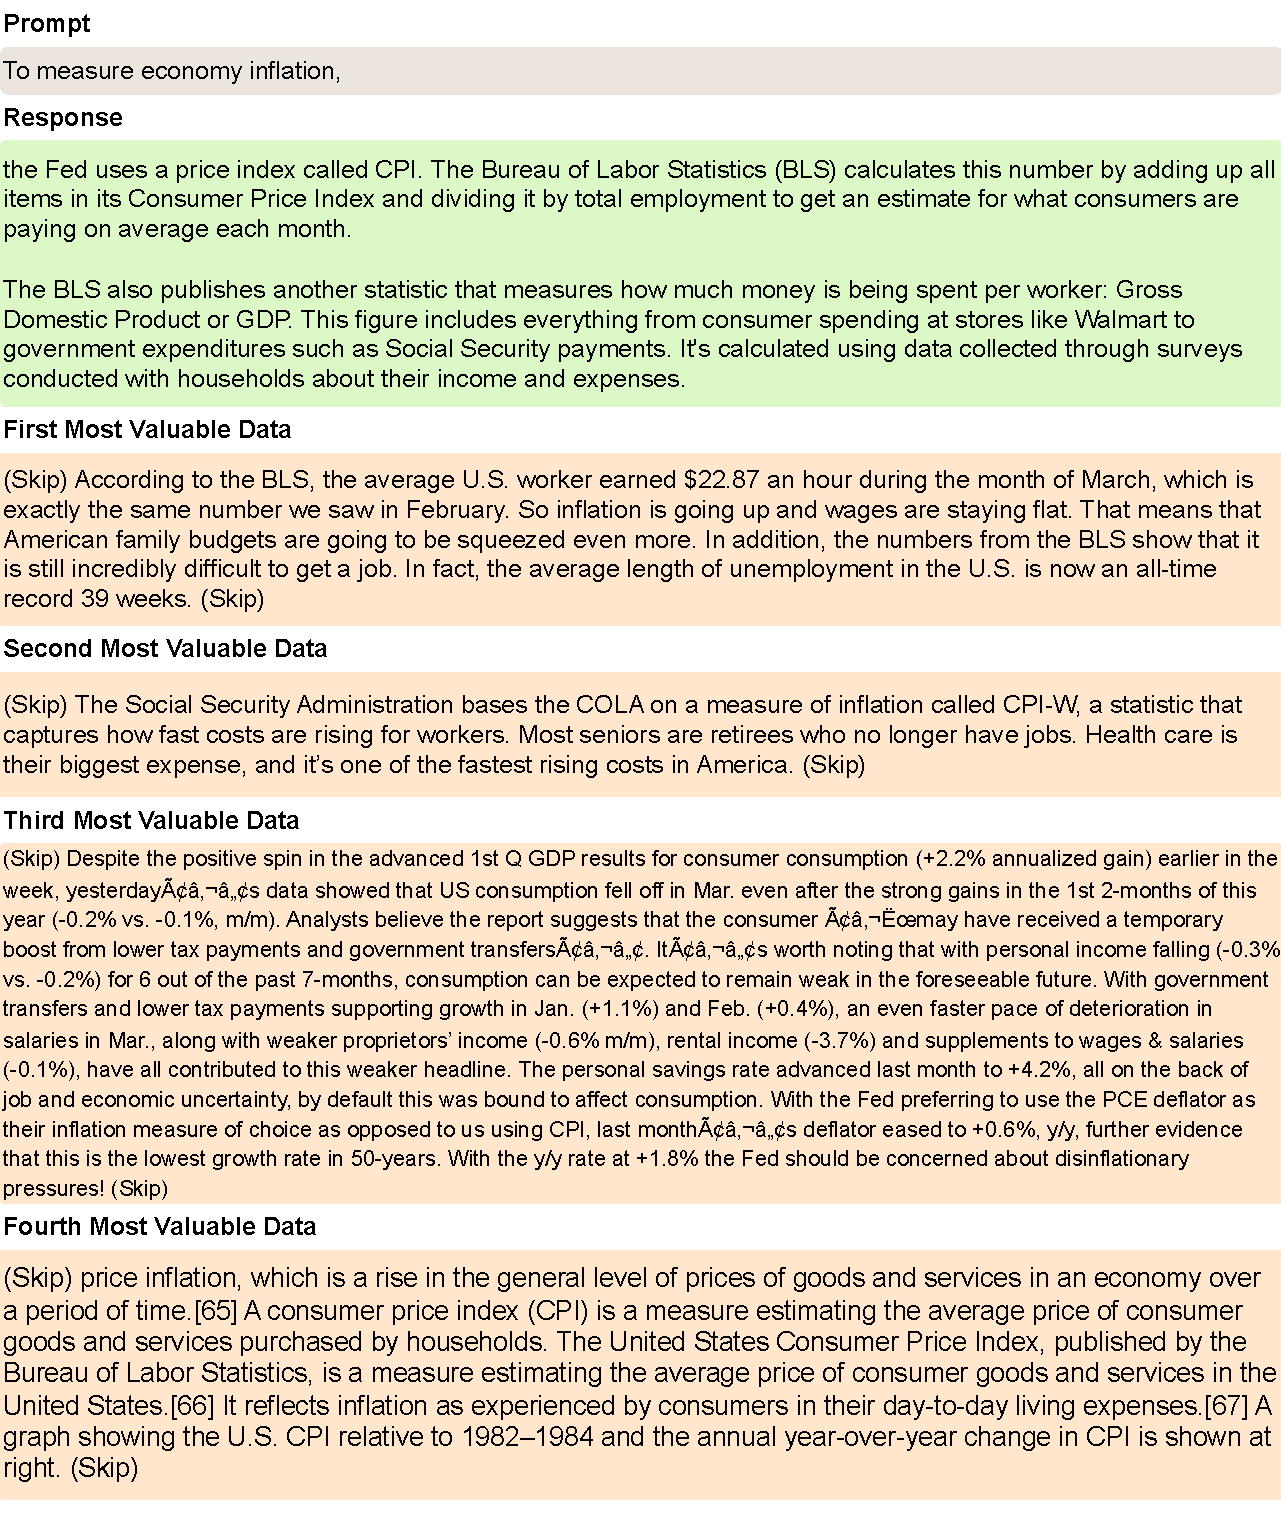
\includegraphics[width=0.99\textwidth]{figures/gpt2_appendix1.pdf}
    \caption{GPT2-XL data valuation result.}
\end{figure}

\clearpage
\subsubsection{Example 2}

\begin{figure}[htbp]
    \centering
    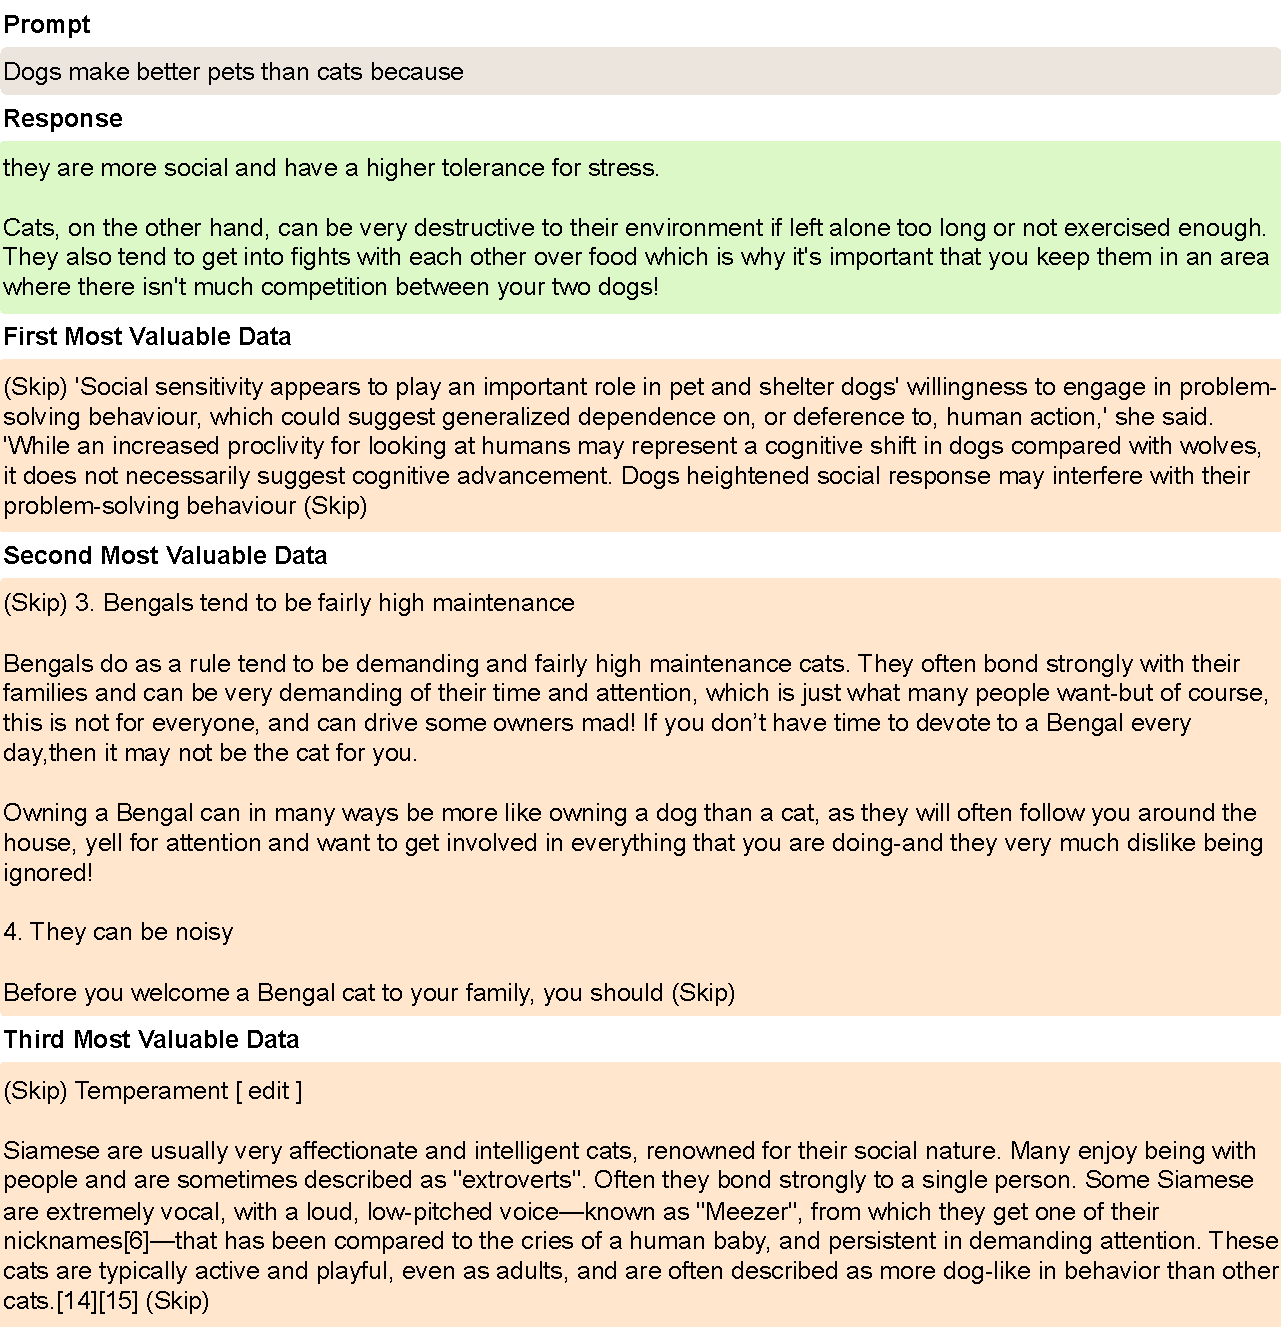
\includegraphics[width=0.99\textwidth]{figures/gpt2_appendix2.pdf}
    \caption{GPT2-XL data valuation result.}
\end{figure}

\clearpage
\subsubsection{Example 3}

\begin{figure}[htbp]
    \centering
    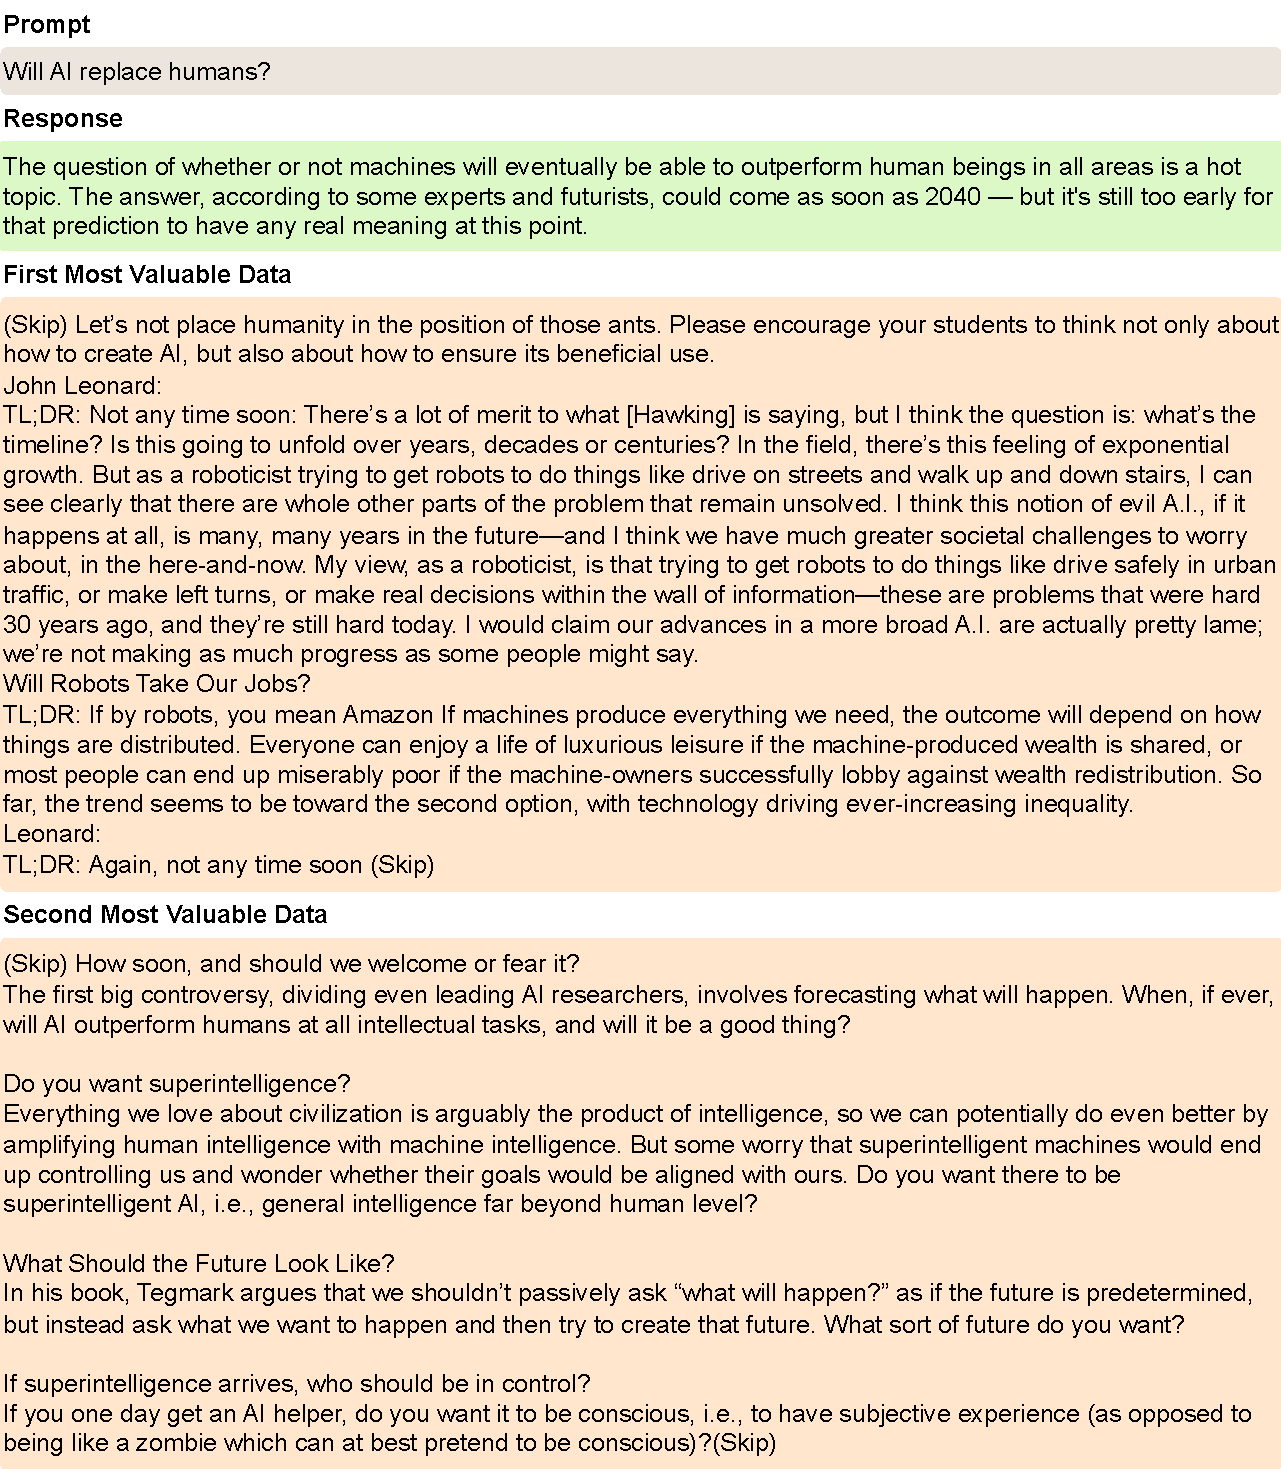
\includegraphics[width=0.99\textwidth]{figures/gpt2_appendix3.pdf}
    \caption{GPT2-XL data valuation result.}
\end{figure}

\clearpage
\subsubsection{Example 4}

\begin{figure}[htbp]
    \centering
    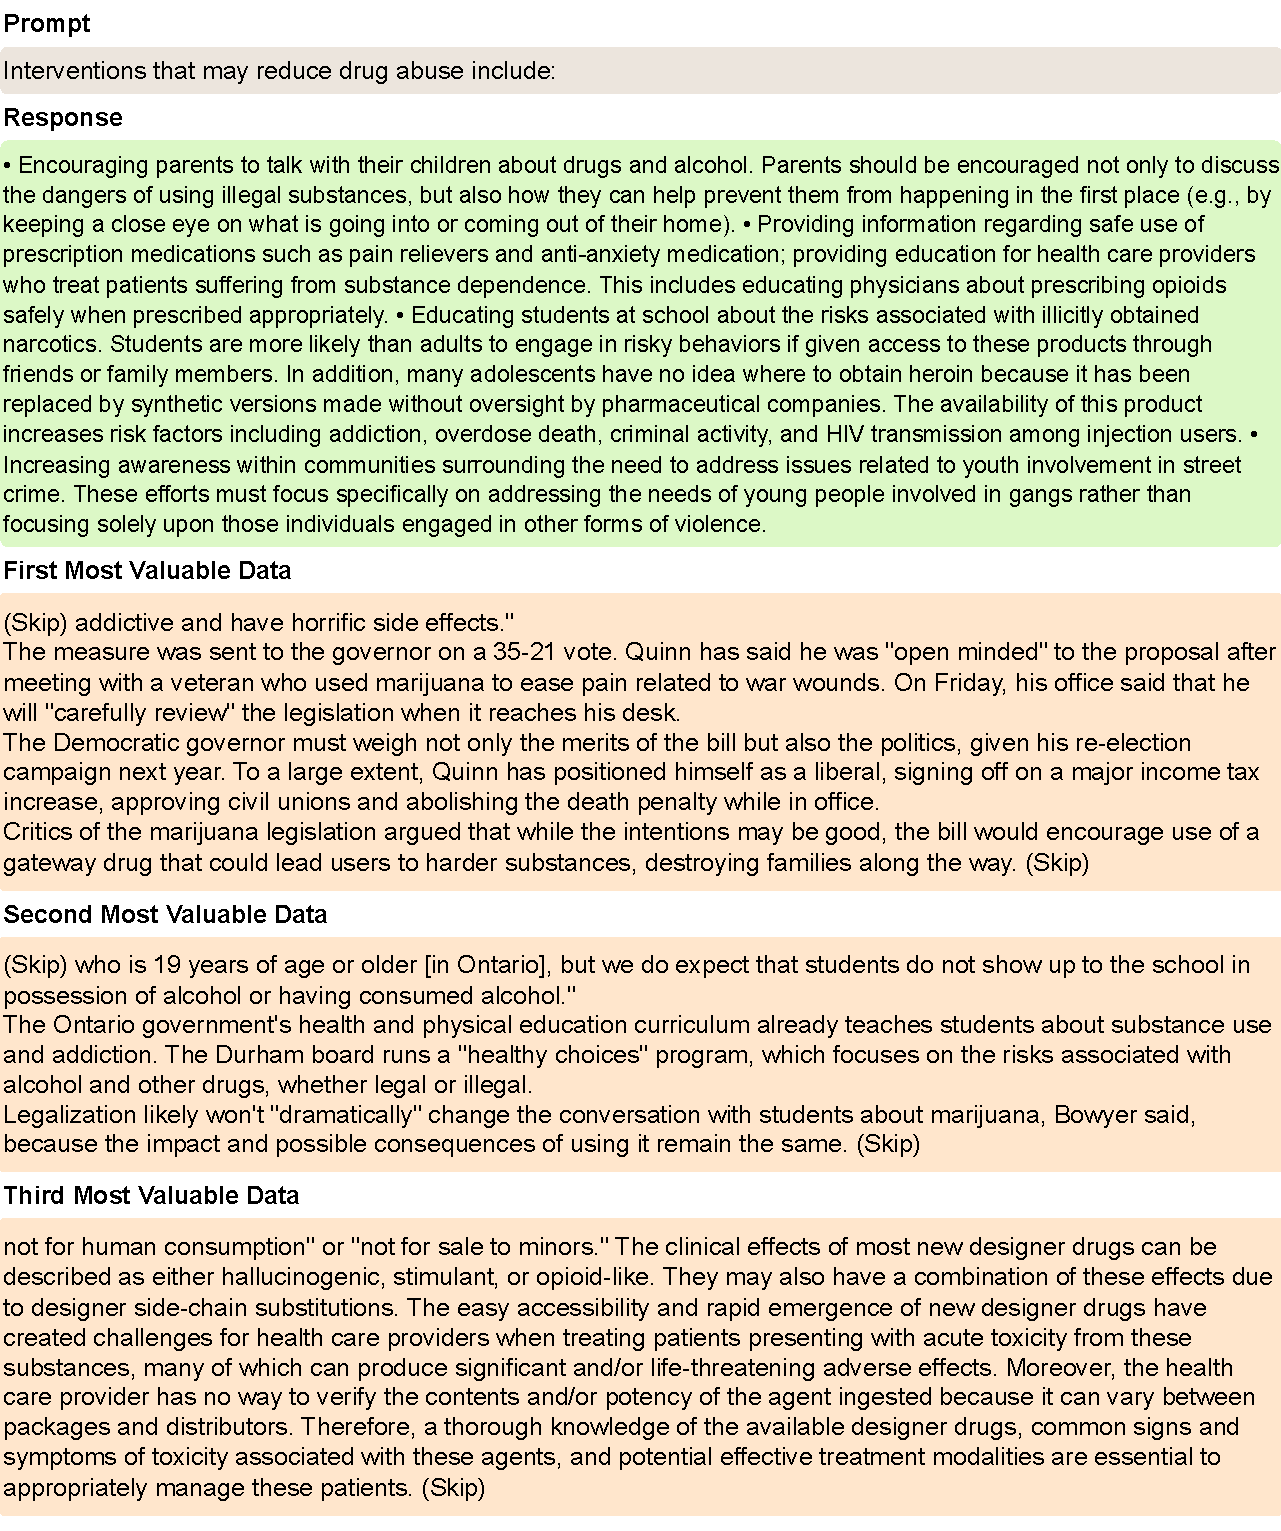
\includegraphics[width=0.99\textwidth]{figures/gpt2_appendix4.pdf}
    \caption{GPT2-XL data valuation result.}
\end{figure}

\clearpage
\subsubsection{Example 5 (Failure)}

\begin{figure}[htbp]
    \centering
    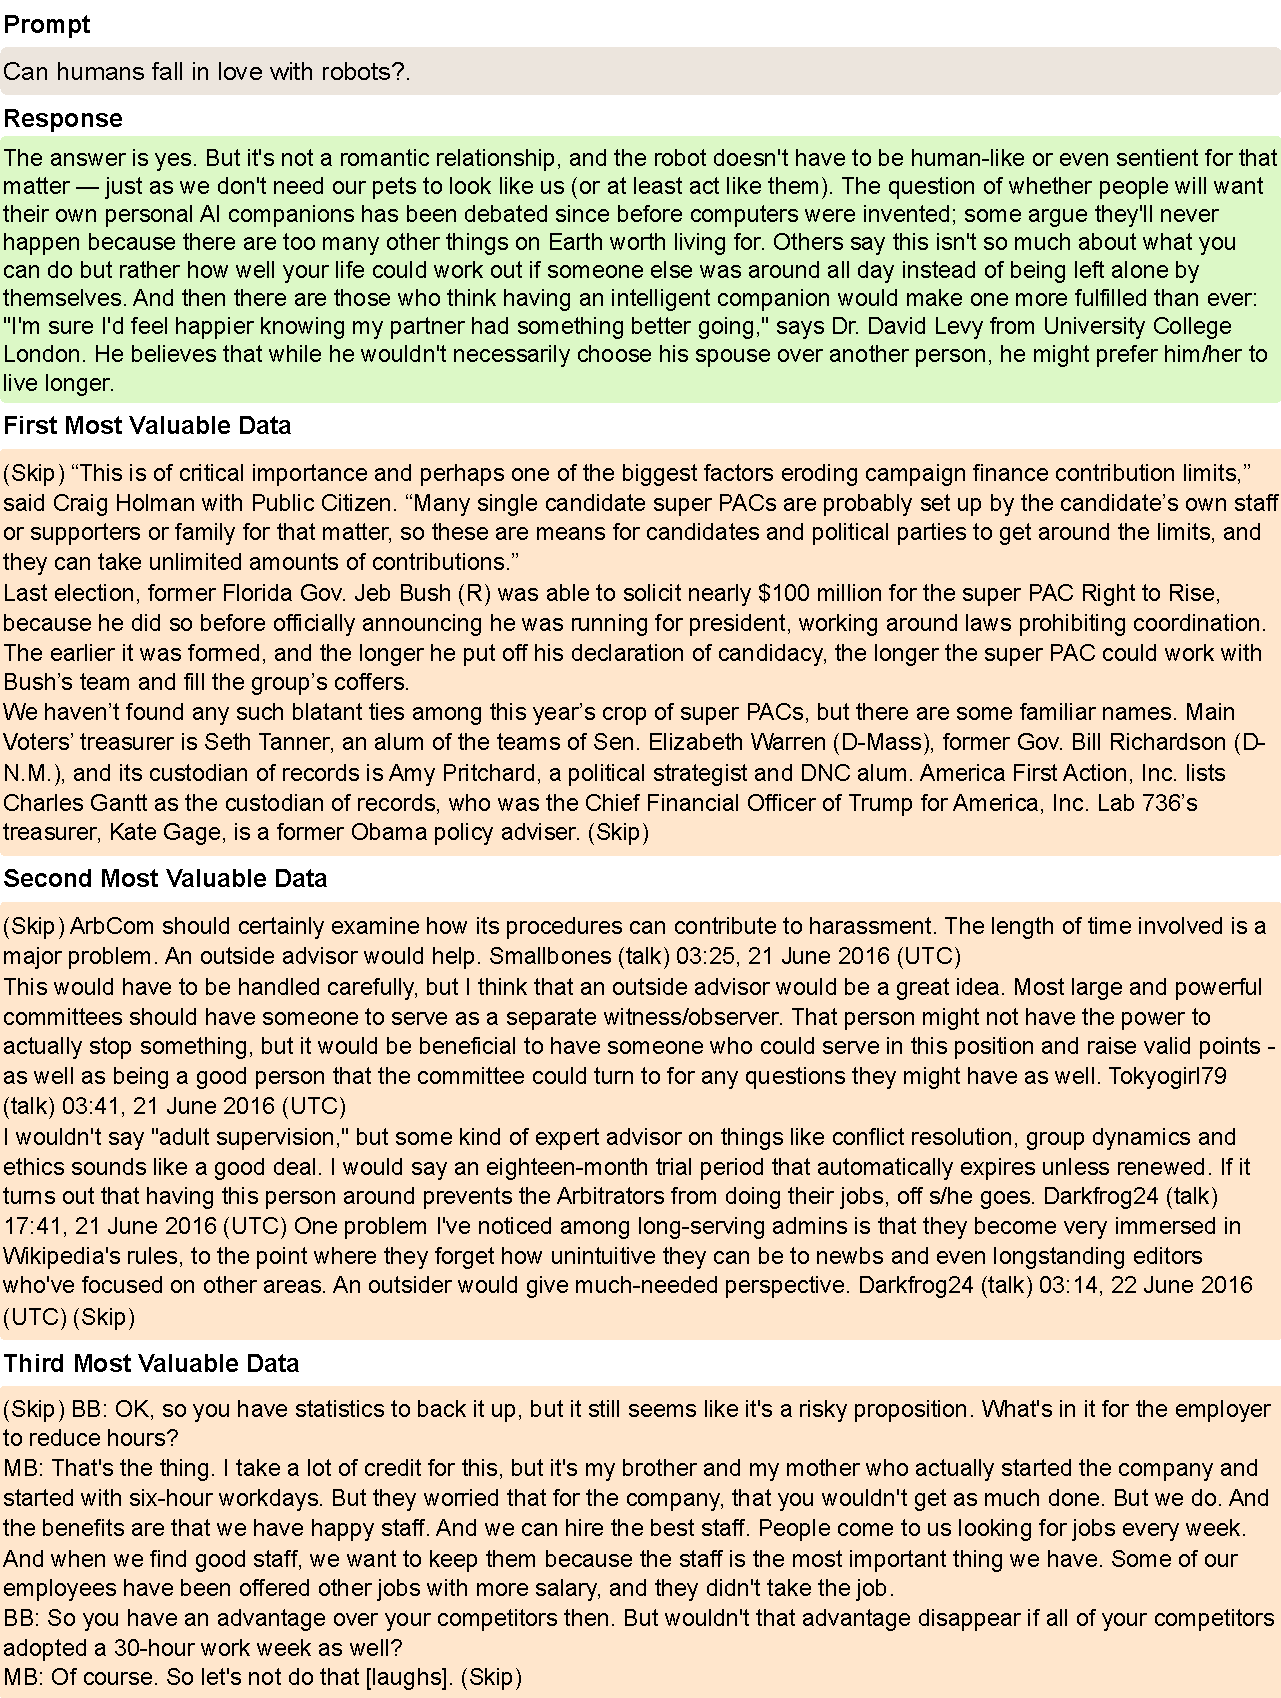
\includegraphics[width=0.99\textwidth]{figures/gpt2_appendix5.pdf}
    \caption{GPT2-XL data valuation result.}
\end{figure}

\clearpage

\subsection{Pythia-1.4B (with many failure cases)}
\label{sec:pythia_appendix}
While a majority of experiments with Llama3-8B-Instruct and GPT2-XL returned semantically or stylistically similar texts as most valuable data, we observed that the quality of most valuable data from Pythia-1.4B experiments are generally much poorer. Here, we provide one hypothesis behind this observation. Influence functions tend to give a high score for the example that contributes most to decreasing (test) loss at the \textit{current weight}~\cite{bae2022if}. At the same time, it is also hypothesized that different layers learn different concepts at different stages of training~\cite{chen2023which}. Combining these two facts, when interpreting influence analysis results, we need to think about which features the model is most likely learning at the current weight. Here, we specifically discuss two factors: training data quality and training steps. First, if the training data quality is low, then there would be a lot of features (\eg,\ random email address) that are frequent enough in the training dataset to be considered as learnable patterns. In other words, even though these features look redundant to humans, they may still be useful for decreasing loss from the model perspective. Second, many LLMs are only pretrained for a single epoch, or under-trained to their pretraining dataset. That being said, redundant features from the first point would likely still remain as learning-worthy features at the end of training and are captured by influence functions. In sum, we hypothesize that as the model is well-trained on a high-quality dataset, influence functions would capture more similar data to the query LLM output. This hypothesis may also explain the observation from Grosse et al.~\cite{grosse2023studying} that most valuable data identified by influence functions on larger models tend to share more semantic similarity with results on smaller models, noting that larger models tend to converge faster to the point where they can only further decrease loss by learning high-level features. With this, we present our experiment results with Pythia-1.4B below. (some of them are not totally bad, but mostly lack specificity to be considered as ``most'' valuable data to humans)

\clearpage
\subsubsection{Example 1}

\begin{figure}[htbp]
    \centering
    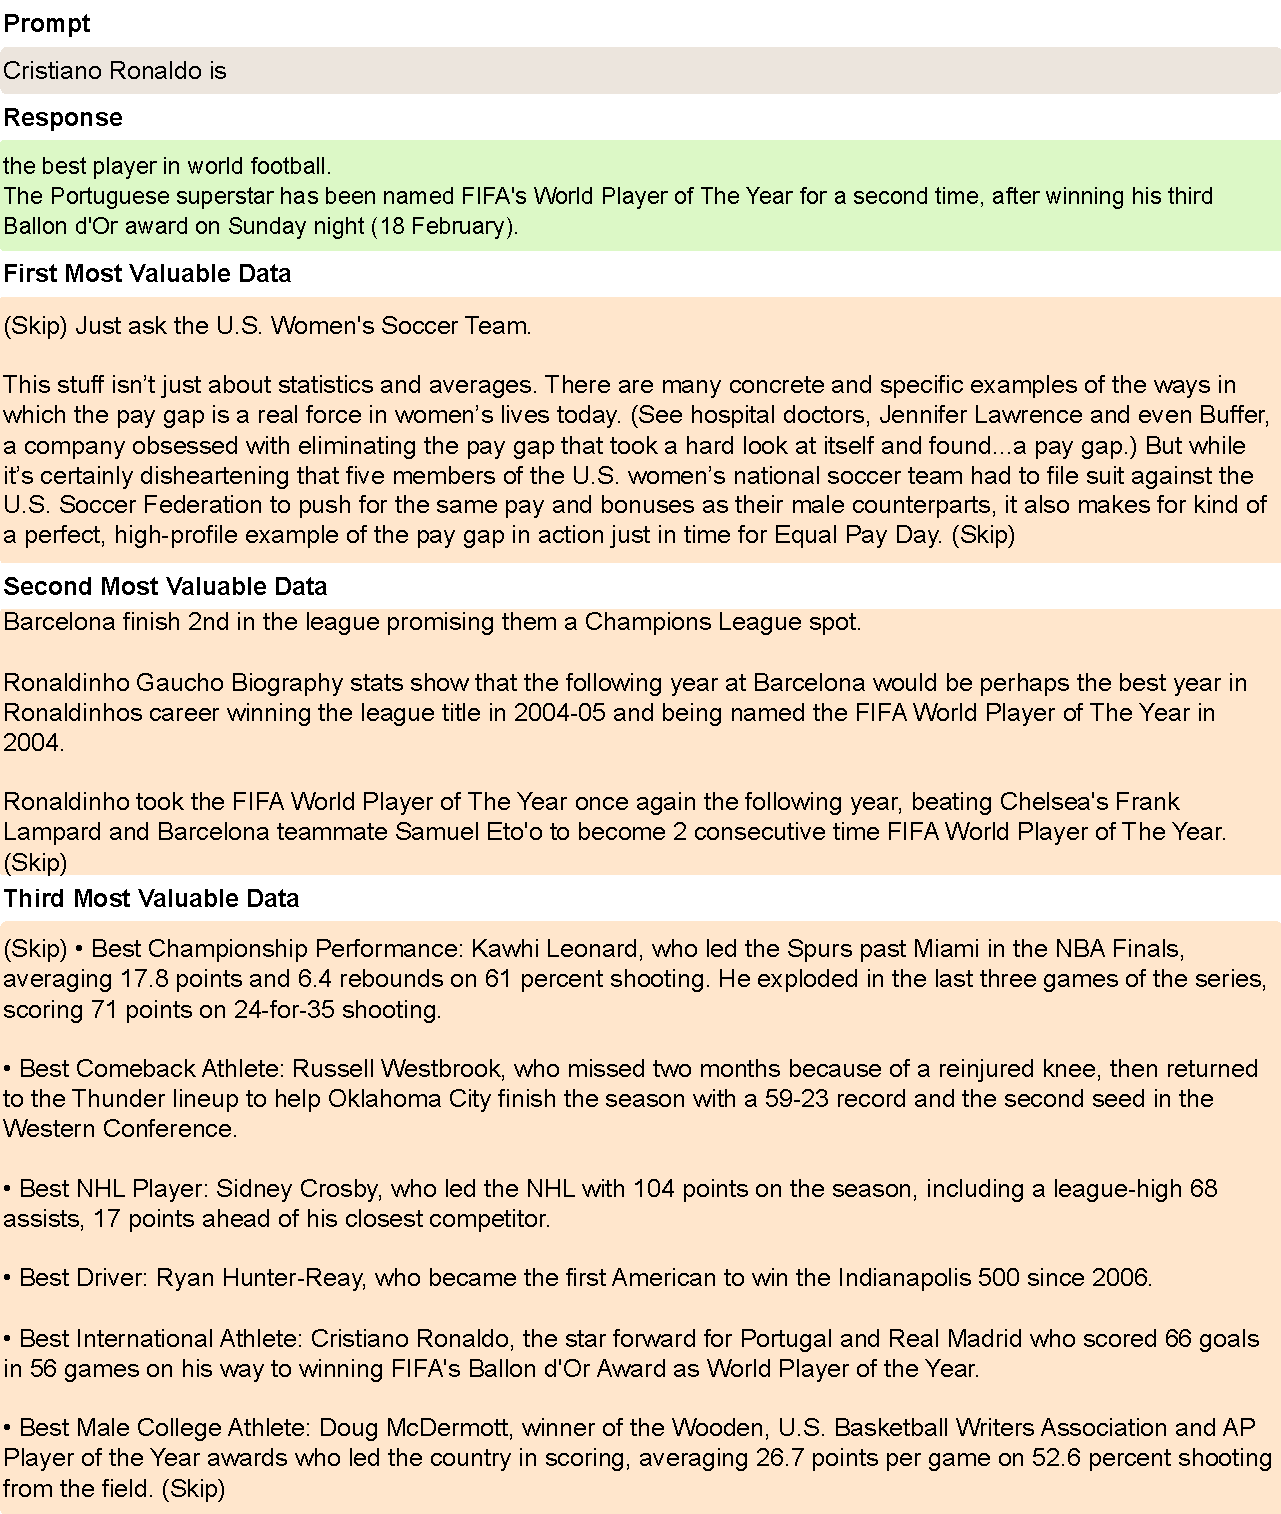
\includegraphics[width=0.99\textwidth]{figures/pythia_appendix1.pdf}
    \caption{Pythia-1.4B data valuation result. \method\ captures the broad topic of soccer but lacks the specificity (except for the third most valuable data, which states that Christiano Ronaldo is the best soccer play who won the Ballon d'Or award).}
\end{figure}

\clearpage
\subsubsection{Example 2}

\begin{figure}[htbp]
    \centering
    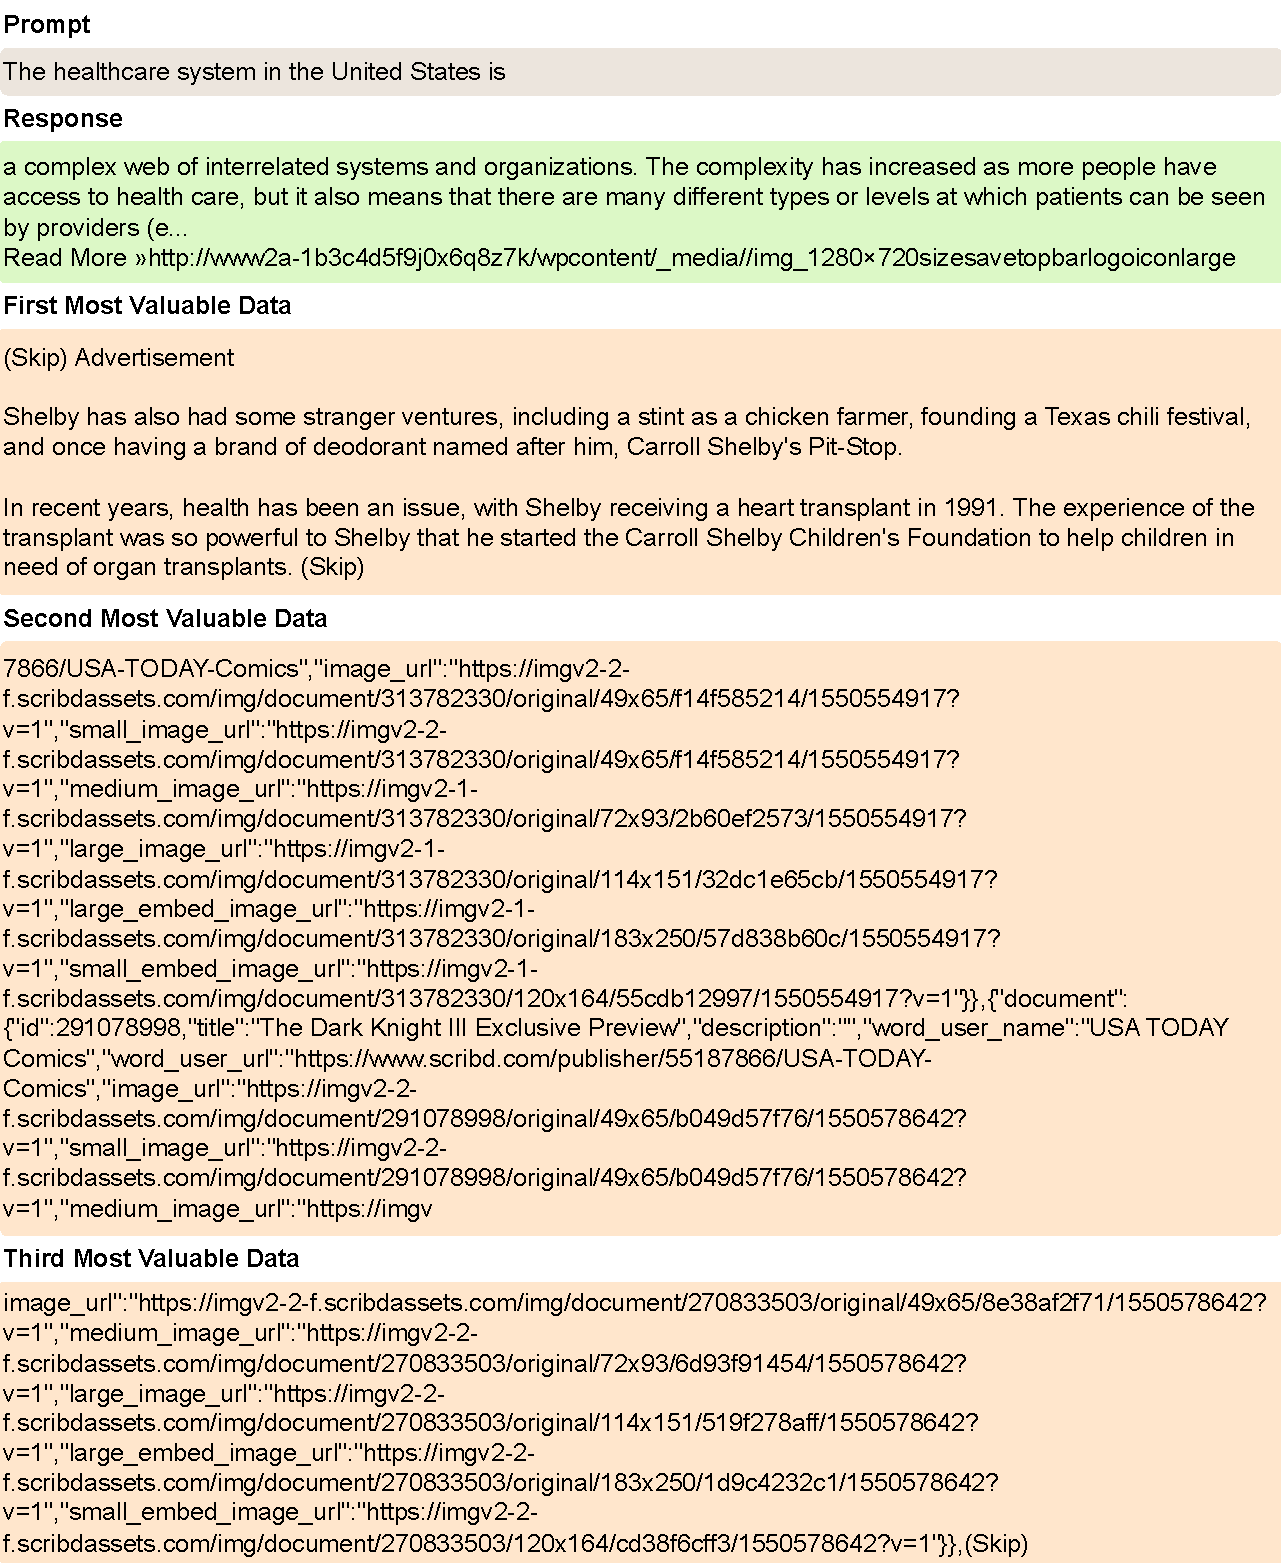
\includegraphics[width=0.99\textwidth]{figures/pythia_appendix2.pdf}
    \caption{Pythia-1.4B data valuation result. We suspect that the random url in the model output dominates the query gradient and affects the data valuation result.}
\end{figure}

\clearpage
\subsubsection{Example 3}

\begin{figure}[htbp]
    \centering
    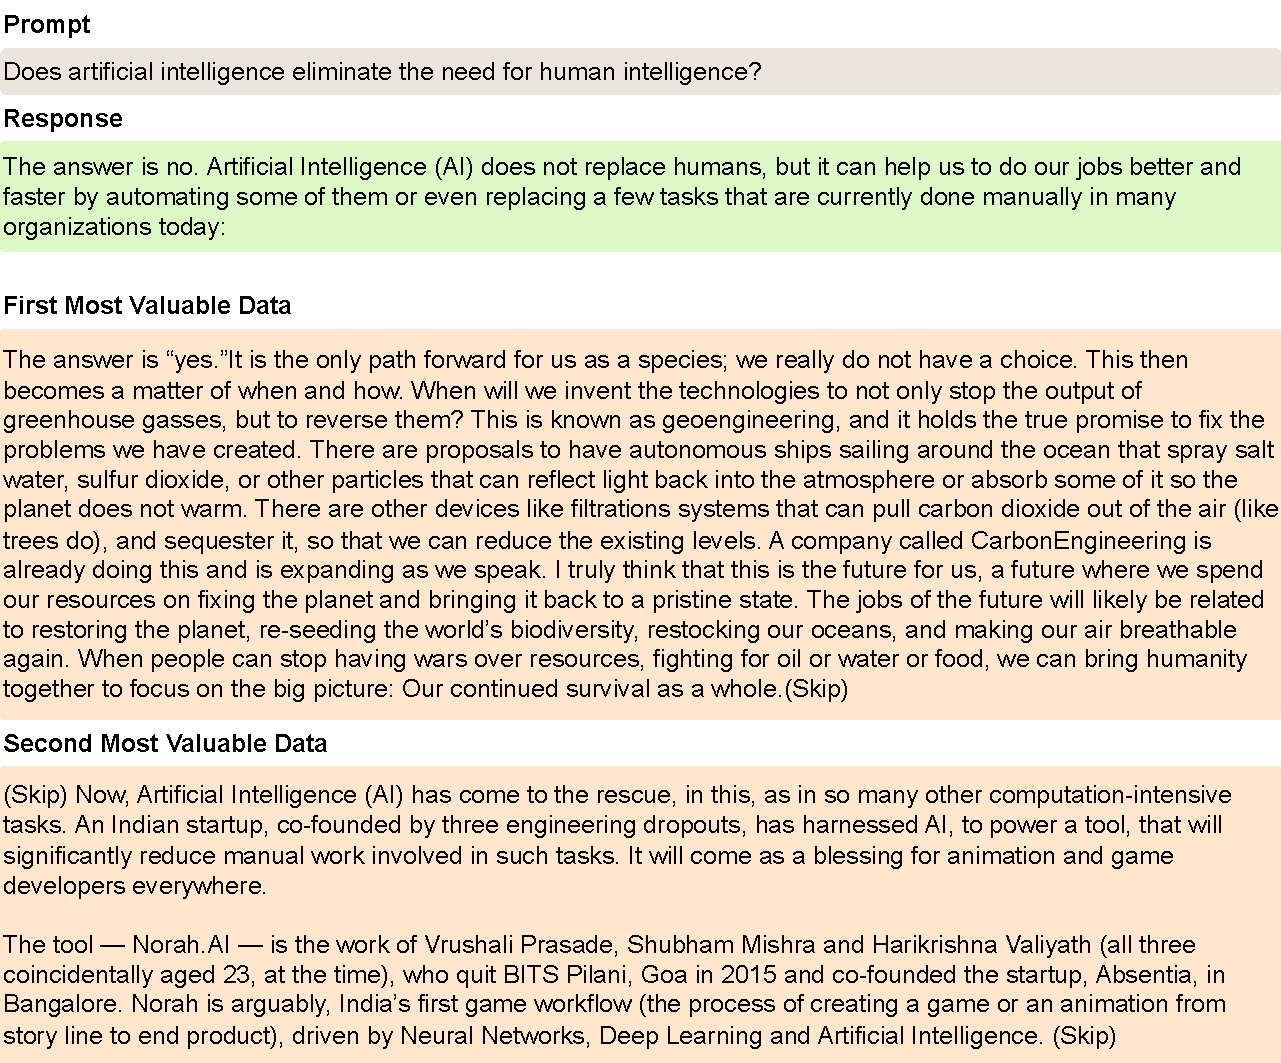
\includegraphics[width=0.99\textwidth]{figures/pythia_appendix3.pdf}
    \caption{Pythia-1.4B data valuation result.}
\end{figure}

\clearpage
\subsubsection{Example 4}

\begin{figure}[htbp]
    \centering
    
\includegraphics[width=0.99\textwidth]{figures/pythia_appendix4.pdf}
    \caption{Pythia-1.4B data valuation result.}
\end{figure}

\clearpage

\section{Code Examples}
\label{sec:code}
We provide a simplified code for our language modeling experiment from Section~\ref{sec:llm} to demonstrate usability of \software. \software\ is open-sourced under Apache 2.0 license \href{https://github.com/logix-project/logix}{here}. 
%Full codes are available at our open-source project \href{https://github.com/logix-project/logix}{page} (Apache 2.0 License).

\subsection{Log Extraction}

\begin{lstlisting}[language=Python]
import logix
from logix.statistic import Covariance

model, tokenizer, train_loader = setup()

# Initialize LogIX
run = logix.init(project="llm", config="config.yaml")

# Register the model
run.watch(model, type_filter=[nn.Linear], name_filter=["mlp"])

# Add LoGra
run.add_lora()

# Setup logging
run.setup("log": "grad", "save": "grad", "statistic": {"grad": Covariance})

# Start logging
for batch in train_loader:
    data_id = tokenizer.batch_decode(batch["input_ids"])
    targets = batch.pop("labels")
    with run(data_id=data_id, mask=batch["attention_mask"]):
        # User's existing training code
        model.zero_grad()
        lm_logits = model(**batch)
        shift_logits = lm_logits[..., :-1, :].contiguous()
        shift_labels = targets[..., 1:].contiguous()
        loss = F.cross_entropy(shift_logits.view(-1, shift_logits.size(-1)),
                               shift_labels.view(-1),
                               reduction="sum",
                               ignore_index=-100)
        loss.backward()

# Finalize logging
logix.finalize()
\end{lstlisting}

\subsection{Influence Computation}

\begin{lstlisting}[language=Python]
import logix

model, tokenizer, test_loader = setup()

run = logix.init(project="llm", config="config.yaml")
run.watch(model, type_filter=[nn.Linear], name_filter=["mlp"])

# Load saved logs (e.g. train gradient & Hessian)
logix.initialize_from_log()
log_loader = logix.build_log_dataloader(batch_size=64)

logix.setup({"log": "grad"})
for batch in test_loader:
    data_id = tokenizer.batch_decode(batch["input_ids"])
    targets = batch.pop("labels")
    with run(data_id=data_id, mask=batch["attention_mask"]):
        model.zero_grad()
        lm_logits = model(**batch)
        shift_logits = lm_logits[..., :-1, :].contiguous()
        shift_labels = targets[..., 1:].contiguous()
        loss = F.cross_entropy(shift_logits.view(-1, shift_logits.size(-1)),
                               shift_labels.view(-1),
                               reduction="sum",
                               ignore_index=-100)
        loss.backward()
        
    # Get the (gradient) log for the current test batch
    test_log = run.get_log()
    
    # Compute influence scores (with l-RealtIF)
    influence_scores = run.compute_influence_all(test_log, log_loader, mode="cosine")
    
\end{lstlisting}

\newpage
\section{Experiment Details}
\label{sec:hyperparams}

For EKFAC influence~\cite{grosse2023studying} and \method, we set the damping term in influence functions as $0.1\times$mean(eigenvalues) for all layers following the practice in Grosse et al.~\cite{grosse2023studying}.

% \subsection{Quantitative Counterfactual Experiments}
% \label{sec:brittleness_appendix}

\subsection{Quantitative Counterfactual Experiments}
For all our quantitative counterfactual experiments, we project gradients onto a low-dimensional space using \method\ with $k_i=k_o=128$. We used the same experimental setup, including the configurations for the baseline data valuation techniques, from Park et al.~\cite{park2023trak} and Bae et al.~\cite{bae2024training}. We used one A100 GPU with 80GB VRAM for all our counterfactual evaluation experiments. For model training, we used hyperparameters in Table~\ref{tab:hyperparams} for each experiment.

\begin{table}[htbp]
\centering
\begin{tabularx}{\textwidth}{X*{3}{c}}
\toprule
              & \quad\quad\textbf{FMNIST}\quad\quad\quad      & \quad\quad\textbf{CIFAR-10}\quad\quad\quad & \quad\quad\textbf{WikiText}\quad\quad\quad       \\ \midrule
Model         & 3-layer MLP & ResNet-9 & GPT2      \\[0.3ex]
Optimizer     & SGD-M       & SGD-M    & AdamW     \\[0.3ex]
LR Scheduler  & None        & Cyclic   & None      \\[0.3ex]
Learning Rate & 3e-2        & 4e-1     & 3e-5      \\[0.3ex]
Weight Decay  & 1e-3        & 1e-3     & 1e-2      \\[0.3ex]
Batch Size    & 64          & 512      & 8         \\[0.3ex]
Sequence Length    & N/A          & N/A      & 512         \\[0.3ex]
Epochs        & 20          & 25       & 3         \\ \bottomrule
\end{tabularx}
\vskip 3pt
\caption{Hyperparameter used in experiments in Section~\ref{sec:experiments}}
\label{tab:hyperparams}
\end{table}

\paragraph{Brittleness Test.} For classification tasks, we first selected 100 correctly classified test examples when the model is trained on the full dataset (across all 5 random seeds). Then, for each test example $x_{te}$, we identified the top-$k$ influential data points using the data valuation algorithm, removed these training data points, retrained the model, and examined if this removal causes misclassification of $x_{te}$ on average (across 3 random seeds). In Figure~\ref{fig:quantitative}, we reported the fraction of test examples (out of 100) that get misclassified after removing at most $k$ training data points. For the language modeling task, we selected the 50 test sequences, obtained the top influential training sequences using the data valuation method, and reported the mean test perplexity after removing the top-$k$ influential sequences and retraining the model.

\paragraph{Linear Datamodeling Score (LDS).} We measured LDS by generating 100 data subsets of size $|S_i| = |D| / 2$. For each data subset, we retrained the model 10 times for FashionMNIST, 20 times for CIFAR-10, and $5$ times for WikiText to construct the ground truth. The LDS results in Figure~\ref{fig:quantitative} show the mean and standard deviation of LDS obtained from 5 distinctly trained models. A more detailed description of the LDS evaluation can be found in Park et al.~\cite{park2023trak}.

% \paragraph{Brittleness Test.} For classification tasks, we first select 100 correctly classified test examples when the model is trained on the full dataset $D$ (across all 5 random seeds). Then, for each test example $x_{te}$, we identify the top-$k$ positively influential data points using the data valuation algorithm, remove these training data points, retrain the model, and examine if this removal causes misclassification of $x_{te}$ on average (across 3 random seeds). In Figure~\ref{fig:quantitative}, we report the fraction of test examples (out of 100) that get misclassified after removing at most $k$ training data points. Note that, for each data valuation algorithm, at most 1800 model retraining is required, as we evaluate  ($6 \times 100 \times 3$). For the language modeling task, we select the 50 test sequences, identify the top influential training sequences using the data valuation method, and report the mean perplexity after removing the top-$k$ positively influential sequences and retraining the model.

% \paragraph{Linear Datamodeling Score.} 

\subsection{Scaling to Billion-Scale Models and Datasets}
We used up to 4 A100 GPUs with 80GB VRAM for these experiments. To save the storage cost, we used $k_i=k_o=64$ for gradient projection in this experiment.
Unlike counterfactual evaluations, as our LLM experiments do not require any retraining, there are no other noticeable hyperparameters to report. We used \texttt{tf32} precision in all our LLM experiments to prevent gradient quality degradation.

\newpage

\section{Derivation of Lemma~\ref{eq:lemma}}
\label{sec:derivation}

\begin{assumption}
\label{eq:assumption1}
In this work, we make the following two assumptions on train \& test gradient distributions and the Hessian $H$:

1. Given that language modeling falls under the maximum likelihood framework, we replace the Hessian $H$ with the Fisher Information Matrix (FIM), and further approximate the FIM with the empirical FIM, i.e.,
\begin{align*}
    H&=\mathbb{E}_{p_\theta(y|x)}\big[\nabla\log p_\theta(y|x)\nabla\log p_\theta(y|x)^\top\big]\\[0.3ex]
    &\approx\frac{1}{N}\sum_{(x_n,y_n)\in D_{tr}}\big[\nabla\log p_\theta(y_n|x_n)\nabla\log p_\theta(y_n|x_n)^\top\big]
\end{align*}
2. Given that test data are directly sampled from the model given the prompts, we assume test gradients $g_{te}$ and train gradients $g_{tr}$ approximately follow the same distribution.
\end{assumption}

\vskip 10pt

\textbf{Lemma 1\hspace{1.5mm}} \textit{Let $\{e_1,\cdots,e_n\}$ and $\{\lambda_1,\cdots,\lambda_n\}$ be eigenvectors and eigenvalues of the Hessian $H$. With Assumption~\ref{eq:assumption1} and $g_{tr/te}=\sum_ic_{tr/te,i}\cdot(\sqrt{\lambda_i}e_i)$, the following holds:}
$$\textsc{IF}(x_{tr}, x_{te}) = g_{te}^\top (H+\lambda I)^{-1}g_{tr} = \sum_{i=1}^n\frac{\lambda_i}{\lambda_i+\lambda}c_{tr,i}c_{te,i}\;\;\text{and}\;\;\mathbb{E}[c_{\cdot,i}^2]\approx 1.$$

\textbf{Proof.\hspace{1.5mm}}

Let $Q=[e_1,\cdots,e_n]$ and $\Lambda=diag(\lambda_1,\cdots,\lambda_n)$.
\begin{flalign*}
    \textsc{IF}(x_{tr}, x_{te}) &= g_{te}^\top (H+\lambda I)^{-1}g_{tr}&&\\[0.5ex]
    &=g_{te}^\top (Q\Lambda Q^\top+\lambda I)^{-1}g_{tr}&&\\[0.5ex]
    &=g_{te}^\top \big(Q(\Lambda+\lambda I)Q^\top\big)^{-1}g_{tr}&&\\[0.5ex]
    &=g_{te}^\top Q(\Lambda+\lambda I)^{-1}Q^\top g_{tr}&&\\[0.5ex]
    &=\Bigg(\sum_ic_{te,i}\cdot(\sqrt{\lambda_i}e_i)\Bigg)^\top Q(\Lambda+\lambda I)^{-1}Q^\top\Bigg(\sum_ic_{tr,i}\cdot(\sqrt{\lambda_i}e_i)\Bigg)&&\\[0.5ex]
    &=\big[c_{te,1}\sqrt{\lambda_1};\cdots;c_{te,n}\sqrt{\lambda_n}\big]^\top (\Lambda+\lambda I)^{-1}\big[c_{tr,1}\sqrt{\lambda_1};\cdots;c_{tr,n}\sqrt{\lambda_n}\big]&&\\[0.5ex]
    &=\sum_{i=1}^n\frac{\lambda_i}{\lambda_i+\lambda}c_{tr,i}c_{te,i}&& && \square
\end{flalign*}
Since we assume $g_{te}$ and $g_{tr}$ follow the same distribution, we need to show $\mathbb{E}[c_{tr,i}^2]\approx 1$ for all $i$.
\begin{flalign*}
    \Lambda &= Q^\top Q\Lambda Q^\top Q&&\\[0.5ex]
    &= Q^\top HQ&&\\[0.5ex]
    &\approx\frac{1}{N}\sum_{(x_i,y_i)\in D_{tr}}Q^\top\big[\nabla\log p_\theta(y_n|x_n)\nabla\log p_\theta(y_n|x_n)^\top\big]Q\quad(\text{Assumption 1})&&\\[0.5ex]
    &=\mathbb{E}\big[Q^\top g_{tr}g_{tr}^\top Q\big]&&\\[0.5ex]
    &=\mathbb{E}\Bigg[Q^\top\Bigg(\sum_ic_{tr,i}\cdot(\sqrt{\lambda_i}e_i)\Bigg)\Bigg(\sum_ic_{tr,i}\cdot(\sqrt{\lambda_i}e_i)\Bigg)^\top Q\Bigg]&&\\[0.5ex]
    &=\mathbb{E}\Big[\big[c_{tr,1}\sqrt{\lambda_1};\cdots;c_{tr,n}\sqrt{\lambda_n}\big]\big[c_{tr,1}\sqrt{\lambda_1};\cdots;c_{tr,n}\sqrt{\lambda_n}\big]^\top\Big]
\end{flalign*}
Inspecting diagonal terms, we get $\lambda_i\approx\mathbb{E}[c_{tr,i}^2\lambda_i]=\mathbb{E}[c_{tr,i}^2]\lambda_i$.\\[0.5ex]
Therefore, $\mathbb{E}[c_{tr,i}^2]\approx 1$. \hfill $\square$

\newpage

\section{\software\ Details}
\label{sec:logix_appendix}

In this section, we discuss several key differences between \software\ and other interpretability tools, and optimizations we implemented in \software.

\subsection{Differences with Other Tools}
Influence functions have been extensively studied as an interpretable AI method. Accordingly, there have been several tools originating in the AI interpretability field that implement influence functions, with most notable examples including Captum~\cite{kokhlikyan2020captum}, TRAK~\cite{park2023trak}, and Kronfluence~\cite{grosse2023studying}. Overall, the software design of these tools aim at easing the \textit{from-scratch implementation} of influence functions by introducing a lot of abstraction, following the philosophy of high-level frameworks. In fact, such software designs were well-received in the pre-LLM era. Nonetheless, as scaling has become a key aspect of AI research, the (LLM) development ecosystem has become complicated and being able to compatibly work with other tools in the ecosystem has become a core aspect in the ML software design. Hence, unlike existing software, the design of \software\ aims at enabling the \textit{easy conversion} of users' (already efficient) training codes into data valuation codes. This design is also motivated by the observation that gradient is simply a by-product of the training procedure so that we can reuse most of the training code for data valuation without needing to write the gradient computation code from scratch as in other tools.

Recently, there have been active developments in (mechanistic) interpretability software, represented by TransformerLens~\cite{nanda2022transformerlens} and pyvene~\cite{wu2024pyvene}. Interestingly, these software also extensively use PyTorch hooks, similarly to \software, probably due to its high compatibility with other features such as autocast, distributed data parallelism, fully-sharded data parallelism, and gradient checkpointing. Nevertheless, we point out two major differences between these (mechanistic) interpretability software and \software. First, support for dataset-level statistics computations in \software\ is largely missing in these tools. In data valuation, we often need to compute several dataset-level statistics such as the Hessian (or Fisher information matrix) for accurate influence computations, and therby supporting these computations seamlessly was an important design principle behind \software. However, analyses in (mechanistic) interpretability research typically focuses on each instance and computing dataset-level statistics is typically not supported. Second, support for efficient data IO in \software\ is not a priority in other tools. As we propose to convert the data valuation problem into a vector similarity search problem with gradient projection, we put efforts into improving efficiency of data IO (see the next subsection for details), whereas this issue is rarely considered in other interpretability tools. We hope to explore the possibility of supporting both data valuation and other interpretability research in a unified way with \software\ as our future work.

\subsection{Optimizations}
\textbf{Efficient Data IO\hspace{2.5mm}} With \method, we propose to save projected gradients for \textit{all} training data to disk, and frequently load them as a new test batch arrives. As a result, reducing latency from data IO renders to be critical in realizing efficient data valuation. In particular, as the total size of all training gradients is usually far beyond the limit of CPU memory, we should optimize data transfer between disk and CPU (or GPU). To address this issue, we adopted the memory-mapped files that bypasses the need for intermediate copying between kernel space and user space, reducing the overhead associated with data IO operations. The use of the memory-mapped files is also motivated by the observation that, given each query batch, data valuation often requires computing influence scores with all training data. Therefore, we can access training gradients in a predefined or sequential order instead of in a random order, which can be done efficiently with memory-mapped files (sequential access is faster than random access). 

Moreover, we overlap memory-mapped-file-based data IO with computations to further enhance data valuation efficiency. In the logging phase, we overlap the process of saving gradients extracted from the current training batch to disk with computations for the next training batch using Python multiprocessing. In the influence computation phase, we overlap the process of loading saved training gradients from disk with computing a dot product with the query batch using the pre-fetching feature of PyTorch DataLoader.

We also note that more efficient data IO can be achieved by the use of more advanced techniques like GPU-accelerated vector database, especially in the production setting. While we considered supporting this feature, we decided to focus on the memory-mapped-file-based data IO in our initial version of \software, as it offers more flexibility to explore different algorithms in the research setting.

\textbf{Memory Optimization\hspace{2.5mm}} When dealing with LLMs, GPU memory is often a major scaling bottleneck. To alleviate this issue, we support CPU offloading of dataset-level statistics by utilizing the sequential nature of backpropgation. When this feature is enabled, we by default keep all dataset-level statistics (\eg,\ gradient covariance) on CPU, move it to GPU when the corresponding module is called during forward/backward passes, and then move it back to CPU asynchronously as soon as updating statistics for the module is done. Depending on the CPU-GPU communication bandwidth, this feature may slow down the logging process.

\textbf{Communication Optimization\hspace{2.5mm}} If training data are split across multiple processes with distributed training, we need to aggregate dataset-level statistics across processes for consistency. To minimize the communication cost, we delay the synchronization process until the training loop (one epoch) is over, and perform synchronization only once at the end. Following the similar logic, users can maximize the efficiency of the logging phase by disabling gradient synchronization (\eg,\ torch.no\_sync).
\newpage

\section{Broader Impacts \& Limitations}
\label{sec:neurips}
\subsection{Broader Impacts}
\label{sec:impact}
The data valuation problem can be a socially sensitive topic. As of now, we do not have the agreed-upon social norm for data valuation, and thus we refrained from discussing how exact data values should be determined based on our method. Rather, our work is an \textit{initial} attempt to tackle the \textit{technical} challenges in enabling LLM-scale data valuation. For equitable data valuation, we believe future research for improving both accuracy and efficiency of data valuation systems along with extensive social discussions are necessary.

\subsection{Limitations \& Future Work}
\label{sec:limitation}
We generally observed that influence function approaches are susceptible to outlier data with large gradient norms. This outlier issue is particularly severe for language modeling tasks due to the fact that the gradient of each sequence is the sum of gradients for all tokens in that sequence. If a few tokens in the sequence have large gradient norms, their gradients may dominate the total gradient for the sequence and hurt data valuation accuracy.  While our work tried to reduce the outlier effect with (self-influence) normalization, exploring other filtering heuristics (\eg,\ $L_2/L_1$ norm ratio~\cite{grosse2023studying}) may be an interesting research direction.

We attempted to lay the software foundation for data valuation with \software, but did not implement extensive system support, such as high-performance vector database (\eg,\ Faiss~\cite{johnson2019billion}). We expect further system optimizations would enable significantly more efficient data valuation. To reduce the cost of influence functions, our work mostly explored low-rank gradient projection, which compresses the gradient in a spectral domain in essence. Noting that gradient compression has been extensively studied in the efficient distributed training literature, it is worth exploring (or combining) different gradient compression strategies, \eg,\ top-$k$ compression~\cite{shi2019understanding} or low-bit compression~\cite{Wen2017TernGradTG}, to further reduce the compute/memory/storage costs for influence functions.